\documentclass[a4paper,12p]{scrreprt}
\usepackage[left= 2.5cm,right = 2cm, bottom = 4 cm]{geometry}

% Standard Packages
\usepackage[utf8]{inputenc}
\usepackage[ngerman]{babel}
\usepackage[T1]{fontenc}
\usepackage{graphicx, subfig}
\usepackage{subcaption}
\usepackage{fancyhdr}
\usepackage[backend=biber]{biblatex}
\usepackage{listings}
\lstset{
  language=C,                % choose the language of the code
  numbers=left,                   % where to put the line-numbers
  stepnumber=1,                   % the step between two line-numbers.        
  numbersep=5pt,                  % how far the line-numbers are from the code
  backgroundcolor=\color{white},  % choose the background color. You must add \usepackage{color}
  showspaces=false,               % show spaces adding particular underscores
  showstringspaces=false,         % underline spaces within strings
  showtabs=false,                 % show tabs within strings adding particular underscores
  tabsize=2,                      % sets default tabsize to 2 spaces
  captionpos=b,                   % sets the caption-position to bottom
  breaklines=true,                % sets automatic line breaking
  breakatwhitespace=true,         % sets if automatic breaks should only happen at whitespace
  title=\lstname,                 % show the filename of files included with \lstinputlisting;
}
\usepackage{xcolor}
\usepackage{float}
\addbibresource{references.bib}
\usepackage{enumitem}
\usepackage{mathptmx}
%\usepackage{lmodern}
%\usepackage{color}


%Für Usepackage Lisiting -> ermöglicht Code einzufügen:
\lstset{ 
  language=[Sharp]C,
  basicstyle=\small\ttfamily, % Kleine Schriftgröße für den Code
  keywordstyle=\color{blue},
  commentstyle=\color{green!40!black}, % Dunklere Grüntöne für Kommentare
  stringstyle=\color{orange},
  numbers=left,
  numberstyle=\tiny,
  numbersep=5pt,
  breaklines=true,
  showspaces=false,
  showstringspaces=false,
  frame=none,
  rulecolor=\color{black},
  captionpos=b
}



% zusätzliche Schriftzeichen der American Mathematical Society
\usepackage{amsfonts}
\usepackage{amsmath}
\usepackage[colorlinks=true, linkcolor=blue, citecolor=blue, urlcolor=blue]{hyperref}
% Für Abkürzungsverzeichniss
\usepackage[]{acronym}

% Begin des Dokumenntes
\begin{document}

\renewcommand{\thechapter}{\roman{chapter}}

\begin{figure}[h]
    \centering
    
\includegraphics[width = 0.55\textwidth]{img/Image_OTH.jpg}
    \label{fig: OTH Image}
\end{figure}


\begin{center}
    {\Huge {Vertiefung Microcomputertechnik} }
\end{center}

\vspace{2cm}

\noindent\makebox[\linewidth]{\rule{\linewidth}{0.4pt}}
\begin{center}
    {\Huge\textbf{CAN-TO-GO-SYSTEM} }
\end{center}
\noindent\makebox[\linewidth]{\rule{\linewidth}{0.4pt}}

\vspace{2cm}

\begin{center}
    {\Large {Von Michael Graml und Leonard Kreil} }
\end{center}

\vspace{1cm}

\begin{center}
    {\Large {Betruer/Prüfer: Prof. Dr. Stefan Krämer\\

             }}
\end{center}

\vspace{5cm}

\begin{center}
    {\Large Abgabe: 12.02.2024}
\end{center}

\newpage
\pagenumbering{Roman}
%Ab jetzt mit Kopf und Fußzeile
% ============= Kopf- und Fußzeile =============
\pagestyle{fancy}

%
\lhead{}
\chead{}
\rhead{\slshape \leftmark}
%%
\lfoot{VMC}
\cfoot{Michael Graml und Leonard Kreil}
\rfoot{\thepage}
%%
\renewcommand{\headrulewidth}{0.4pt}
\renewcommand{\footrulewidth}{0.4pt}

%\include{02_Sperrvermerk_Erklärung}
%\include{03_Zusammenfassung}
\addsec{Zusammenfassung / Abstract}
\label{sec:zusammenfassung}
Das ist meine Zusammenfassung

\minisec{Abstract}
\label{abstract}

lalalal

%Inhaltsverzeichnis
\section*{Abkürzungsverzeichnis}

\begin{acronym}
    \acro{USB}[USB]{Universal Serial Bus}
    \acro{RS232}[RS232]{Recommended Standard 232}
    \acro{FSM}[RS232]{Finite State Machine}
\end{acronym}

\tableofcontents
\thispagestyle{fancy}
\pagenumbering{arabic} % Wechsel zu arabischen Seitenzahlen
\renewcommand{\thechapter}{\arabic{chapter}} % Ändert die Kapitelnummerierung auf römische Ziffern



%\include{07_CPCOM}
\chapter{Einleitung}
\label{sec:Einleitung}
\noindent Die Arbeit wurde gemeinschaftlich von Michael Graml und Leonard Kreil durchgeführt. Sollten Unterschiede in der Bearbeitung einzelner Abschnitte vorliegen, sind diese in den jeweiligen Kapiteln gekennzeichnet.\\

\begin {centering}
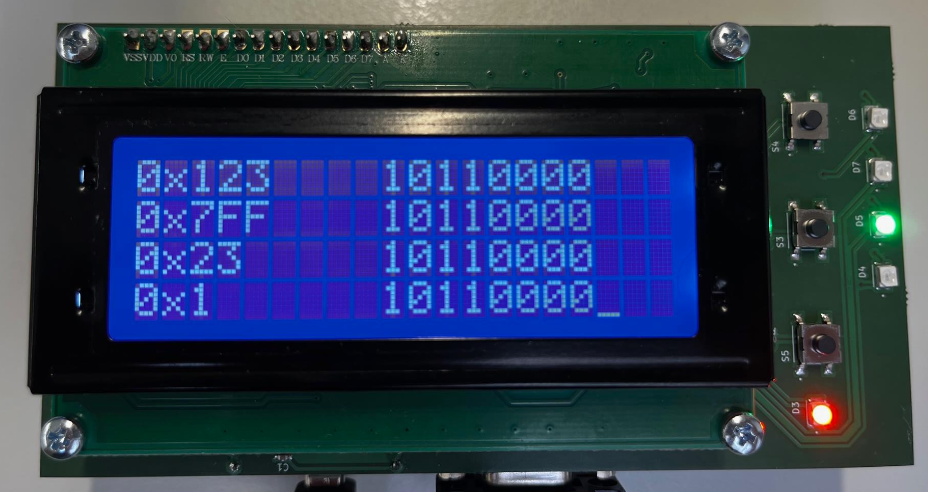
\includegraphics[width=0.75\textwidth]{img/Can_to_go_system.png}
\captionof{figure}{CAN-TO-GO System}
\label{fig: CAN-to-go System}
\end {centering}  


\section{CAN}
Controller Area Network (CAN) ist ein standardisiertes, robustes Fahrzeugbussystem, das für die Kommunikation zwischen verschiedenen Steuergeräten (ECUs) in Fahrzeugen und anderen industriellen Anwendungen konzipiert wurde. Es ermöglicht den zuverlässigen Datenaustausch mit hoher Fehlertoleranz und geringer Latenz, was besonders in Echtzeitanwendungen wichtig ist. CAN-Busse verwenden ein Nachrichtenbasiertes Protokoll, bei dem jede Nachricht eine eindeutige ID hat, die ihre Priorität bestimmt. Dieses System ist besonders nützlich bei der Diagnose von Netzwerkproblemen, da die Priorisierung von Nachrichten und Fehlererkennungsmechanismen die Fehlersuche erleichtern. Die physikalischen Aspekte des CAN-Busses, wie Abschlusswiderstände und die Verkabelung (CANL/CANH), sind ebenfalls entscheidend für die Netzwerkintegrität. Die Anpassungsfähigkeit hinsichtlich der Baudrate und die Unterstützung verschiedener Netzwerkstrukturen machen CAN vielseitig einsetzbar.\\

\section{Can-Datentelegram}
\begin{figure}[h]
    \centering
    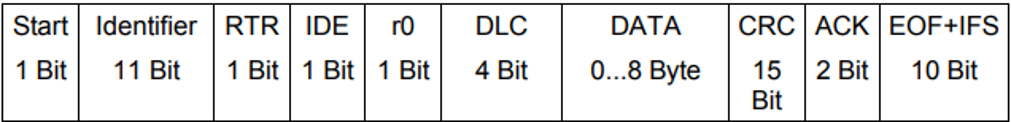
\includegraphics[width = 0.55\textwidth]{img/standard_datenframe.png}
    \caption{Standard Datentelegram \cite{3}}
    \label{fig: Standard Datentelegram}
\end{figure}
\begin{figure}[h]
    \centering
    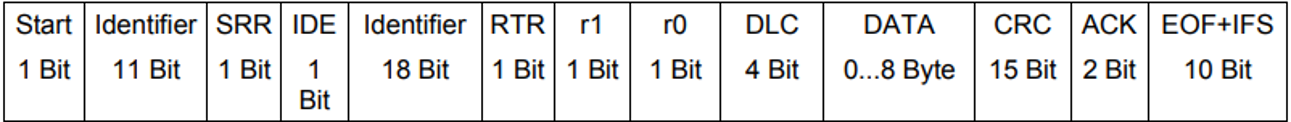
\includegraphics[width = 0.55\textwidth]{img/extended_datenframe.png}
    \caption{Extended Datentelegram \cite{3}}
    \label{fig: Extended Datentelegram}
\end{figure}

\noindent Ein CAN-Datentelegramm beginnt mit einem Startbit zur Synchronisation der kommunizierenden Geräte. Der Identifier gibt die Nachrichtenpriorität an und dient der Busarbitrierung, wobei das RTR-Bit zwischen einem Daten- und einem Datenanforderungstelegramm unterscheidet. IDE ist die Identifier Extension, die anzeigt, ob ein Standard- (11-Bit-Identifier siehe Abbildung \ref{fig: Standard Datentelegram}) oder ein Extended-Frame (29-Bit-Identifier siehe Abbildung \ref{fig: Extended Datentelegram}) verwendet wird. DATA enthält die eigentlichen Nutzdaten. CRC ist eine Prüfsumme zur Fehlererkennung. ACK signalisiert den korrekten Empfang der Nachricht. EOF und IFS kennzeichnen das Ende des Datentelegramms und den erforderlichen Abstand bis zum nächsten Frame. Im Extended Frame ersetzt das SRR-Bit das RTR-Bit des Standard Frames, und die DLC-Information gibt die Länge der Daten an.\\

\section{Anfordderungsanalyse}
\noindent Das "Can to Go"-System wird entwickelt, um Anwendern bei Problemen beim Aufbau eines CAN-Busses zu assistieren und zu diagnostizieren, wo genau die Schwierigkeiten liegen. Es dient als funktionssicherer CAN-Teilnehmer, der in der Lage ist, CAN-Nachrichten zuverlässig zu lesen und zu interpretieren. Kernmerkmale umfassen ein Anschlusskästchen mit SUB-D-Stecker und Status-LEDs, die den Betriebszustand des CAN-Busses anzeigen. Ein optionaler Abschlusswiderstand, der nach Bedarf zugeschaltet werden kann, sowie die Anpassungsfähigkeit der Baudrate gehören ebenfalls zu den wesentlichen Anforderungen. Darüber hinaus wird das System die CAN-Nachrichten und die zugehörigen Sender-IDs sichtbar machen.\\


\section{Endprodukt}

\subsection{Überblick}
\noindent Das Endprodukt des "Can to Go"-Systems bildet eine fortschrittliche Lösung für die Überwachung und Diagnose von CAN-Bussystemen. Es integriert die erforderlichen Funktionen aus der Anforderungsanalyse mit zusätzlichen Merkmalen, die seine Benutzerfreundlichkeit und Vielseitigkeit erhöhen.\\

\subsection{Hauptmerkmale}
\begin{itemize}
    \item \textbf{Anschluss und Konnektivität:} Ausgestattet mit einem Anschlusskästchen und SUB-D-Stecker, verfügt das System über Status-LEDs, die den Betriebszustand des CAN-Busses anzeigen. Diese visuellen Indikatoren erleichtern das schnelle Erkennen von Verbindungsproblemen.
    
    \item \textbf{Funktionalität und Anpassungsfähigkeit:} Ein optionaler Abschlusswiderstand kann nach Bedarf hinzugeschaltet werden. Die Anpassbarkeit der Baudrate gewährleistet eine breite Kompatibilität mit verschiedenen CAN-Bus-Konfigurationen.
    
    \item \textbf{Display und Anzeige:} Das Gerät umfasst ein kleines Display, das CAN-Nachrichten anzeigt. Dieses Display bietet eine direkte, wenn auch begrenzte, Einsicht in die CAN-Kommunikation.
    
    \item \textbf{Energieversorgung:} Es enthält keinen eigenen Akku, kann aber durch eine externe Powerbank mit Energie versorgt werden, was eine flexible Nutzung ermöglicht.
\end{itemize}   

\subsection{Zusätzliche Funktionen}
\begin{itemize}
 \item \textbf{App- und Web-Integration:} Ergänzend zum kleinen Display des Geräts ermöglichen eine App und eine Website die detaillierte Ansicht von CAN-Nachrichten, inklusive Zeitstempeln. Diese digitalen Plattformen erlauben eine umfassende Analyse da sie eine größere Benutzeroberfläche als das Display bieten.
\end{itemize}   



\chapter{Hardwareaufbau und Leiterplattenentwurf}
\label{sec:Hardware}



\noindent Der Hardwareaufbau dieses Projekts basiert auf einer sorgfältig gestalteten Leiterplatte, die alle erforderlichen Hardwarekomponenten integriert. Der Prozess des Leiterplattenentwurfs wurde mittels KiCad, einem Open-Source-Tool für PCB-Design, durchgeführt.\\

\begin {centering}
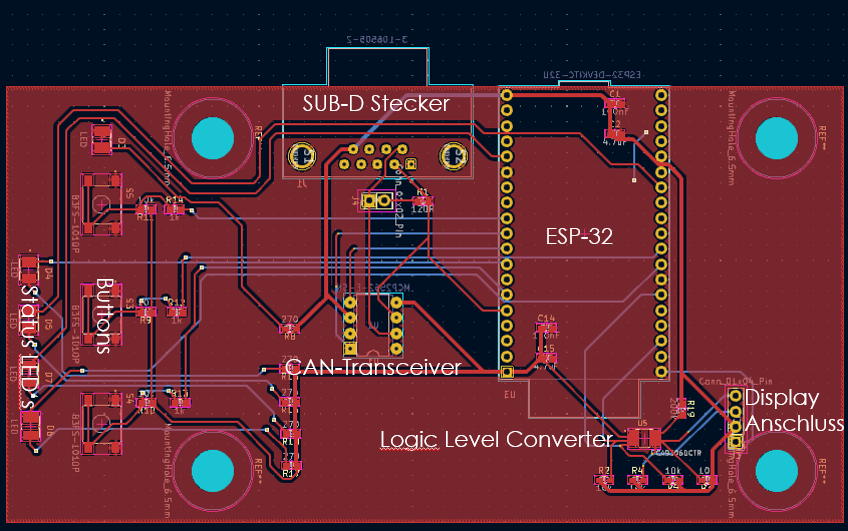
\includegraphics[width=0.75\textwidth]{img/Leiterplate.png}
\captionof{figure}{Leiterplattenentwurf}
\label{fig: Leiterplattenentwurf}
\end {centering}  

\section{Leiterplattenentwurf}
\subsection{Entwurfsprozess}
\begin{itemize}
    \item \textbf{Komponentenauswahl und -platzierung:} Zunächst wurden die benötigten elektronischen Bauteile ausgewählt und in den Schaltplan von KiCad integriert. Jedem Bauteil wurde ein entsprechender Footprint zugewiesen. Diese Footprints sind entscheidend, da sie die physische Größe und Platzierung der Komponenten auf der Leiterplatte bestimmen.
    \item \textbf{Layoutgestaltung:} Im Anschluss wurden die Bauteile sorgfältig auf der Leiterplatte platziert. Besonderes Augenmerk lag dabei auf der logischen Gruppierung der Komponenten und der Minimierung der Leitungslängen, um Effizienz und Signalintegrität zu gewährleisten.
\end{itemize}

\subsection{Herstellung und Bestückung}
\begin{itemize}
    \item \textbf{Leiterplattenbestellung:} Die Leiterplatte wurde bei Aisler in Auftrag gegeben. Die Entscheidung, die Bauteile separat zu bestellen, wurde aus Kostengründen getroffen.
    \item \textbf{Komponentenbeschaffung:} Die einzelnen elektronischen Bauteile wurden von Mouser Electronics bezogen.
    \item \textbf{Bestückung der Leiterplatte:} Die Montage der Bauteile auf der Leiterplatte erfolgte mittels Lötpaste. Bei diesem Prozess wurde besonders auf Präzision und Sauberkeit geachtet, um Kurzschlüsse oder Fehlverbindungen zu vermeiden, die die Funktionalität der Schaltung beeinträchtigen könnten.
\end {itemize}

\noindent Die detaillierte Kostenaufstellung der einzelnen Bauteile sowie der Leiterplatte selbst ist in Tabelle \ref{tab:Stückliste} dargestellt. Diese Übersicht bietet eine klare Kostentransparenz und erleichtert die Nachvollziehbarkeit des Projekts.\\

\section{ESP32}
Der ESP32 ist das Herzstück unseres eingebetteten Systems und übernimmt die zentrale Verarbeitung und Koordination aller Aufgaben. Als hochintegrierter Mikrocontroller verbindet er verschiedene Elemente des Systems, wie die CAN-Schnittstelle, das Display, Status-LEDs und Taster, zu einem funktionierenden Ganzen.\\

\noindent Im Rahmen der CAN-Kommunikation liest der ESP32 die über den CAN-Bus gesendeten Nachrichten und verarbeitet diese. Außerdem steuert ESP32 das Display über das I2C-Protokoll, wobei ein Logikpegelwandler für die Anpassung der unterschiedlichen Spannungsniveaus zwischen dem 3,3-Volt-System des ESP32 und dem 5-Volt-Display verwendet wird.\\

\noindent Die Taster sind über Pull-up-Widerstände an den ESP32 angeschlossen und ermöglichen es den Benutzern, durch einfaches Drücken die Konfigurationseinstellungen vorzunehmen. Der ESP32 interpretiert diese Eingaben und führt die entsprechenden Aktionen aus, wie beispielsweise das Wechseln der Baudrate.\\

\noindent Durch seine Vielseitigkeit und leistungsstarke Verarbeitungskapazität bildet der ESP32 das Rückgrat des Systems.\\

\begin {centering}
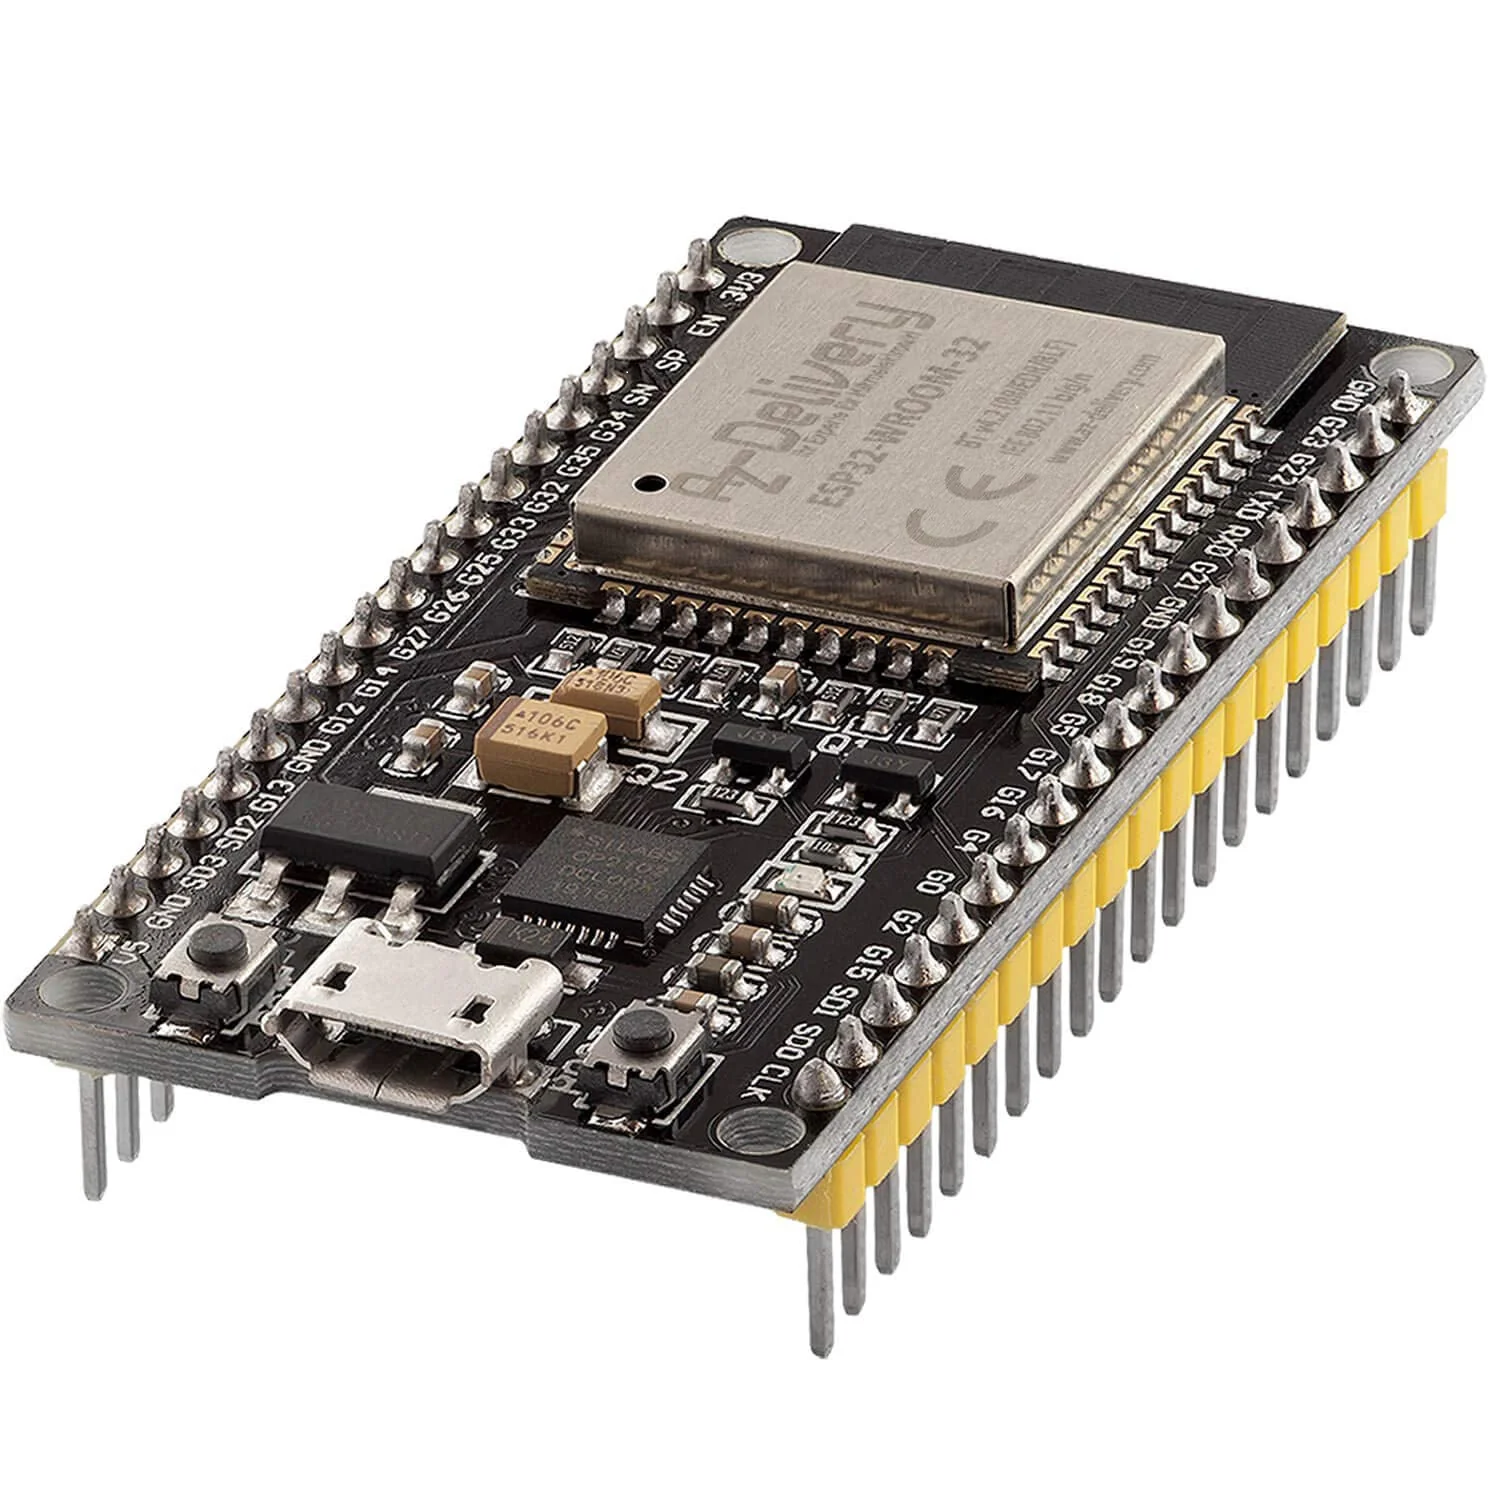
\includegraphics[width=0.5\textwidth]{img/ESP32.png}
\captionof{figure}{ESP32 \cite{1}}
\label{fig: ESP32}
\end {centering}  

\section{Display}
\noindent Das Display dient in unserem eingebetteten System als primäre Benutzerschnittstelle, indem es die Baudrateneinstellungen im Konfigurationsmodus sowie die CAN-Nachrichten und ihre Identifier im Operationsmodus anschaulich visualisiert. In unserem System erfolgt die Kommunikation zwischen dem ESP32-Mikrocontroller und dem Display über das I2C-Protokoll (Inter-Integrated Circuit), einem weit verbreiteten Kommunikationsstandard, der für seine Einfachheit und Effizienz in der synchronen seriellen Datenübertragung bekannt ist.\\

\noindent I2C nutzt nur zwei Leitungen – eine für das serielle Daten-Signal (SDA) und eine für das serielle Clock-Signal (SCL) – und ermöglicht es dem Mikrocontroller, mehrere Geräte über einen einzigen Bus zu steuern, wobei jedes Gerät über eine einzigartige Adresse identifiziert wird. Dieser Bus ermöglicht eine bidirektionale Kommunikation, was bedeutet, dass der ESP32 Daten an das Display senden und gleichzeitig Statusinformationen vom Display empfangen kann. \\

\noindent Da der ESP32 mit einer Logikspannung von 3,3 Volt arbeitet, während das Display für eine Betriebsspannung von 5 Volt ausgelegt ist, wurde ein Logikpegelwandler verwendet, um die Signale zwischen diesen beiden Spannungsebenen zu übersetzen (siehe Abschnitt ...). Zusätzlich wird für die physische Verbindung des Displays ein serieller I2C/TWI-Schnittstellenadapter verwendet, der bereits im Lieferumfang des Kits enthalten ist.\\

\begin{centering}
  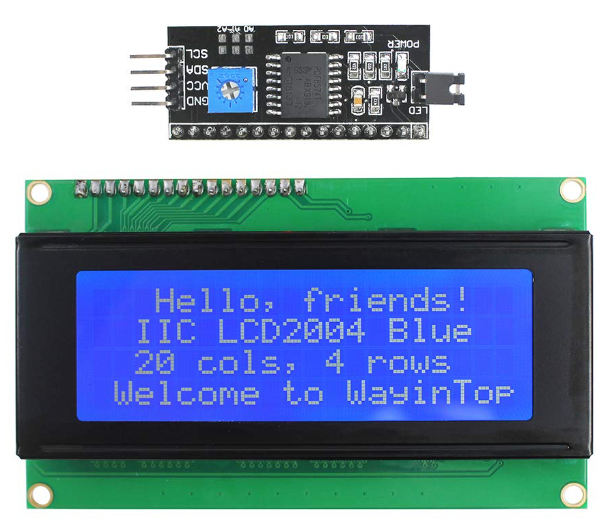
\includegraphics[width=0.5\textwidth]{img/Display.png}
  \captionof{figure}{Display mit Displayanschluss \cite{4}}
  \label{fig: Display}
\end{centering}

\section{SUB-D Stecker}
\noindent Der SUB-D-Stecker dient der Einbindung von CAN-Nachrichten in das betreffende System. Über diese Schnittstelle lässt sich das 'CAN to go'-System mit dem zu testenden CAN-Netzwerk verbinden. Die Konfiguration der Pin-Belegung ist spezifisch angeordnet: CAN-Low ist an Pin 2, CAN-High an Pin 6, der Masseanschluss (GND) an Pin 3 und die Versorgungsspannung von +5V an Pin 9 angebunden. Abhängig von den systemseitigen Erfordernissen kann ein 120-Ohm-Terminierungswiderstand zwischen CAN-Low und CAN-High integriert werden, um die Signalintegrität zu gewährleisten. Die Schaltung dieses Terminierungswiderstandes erfolgt über den Anschluss J4, der in der grafischen Darstellung blau umkreist ist (siehe Abbildung \ref{fig: SUB-D Stecker und Terminierungswiderstand}).\\

\begin{centering}
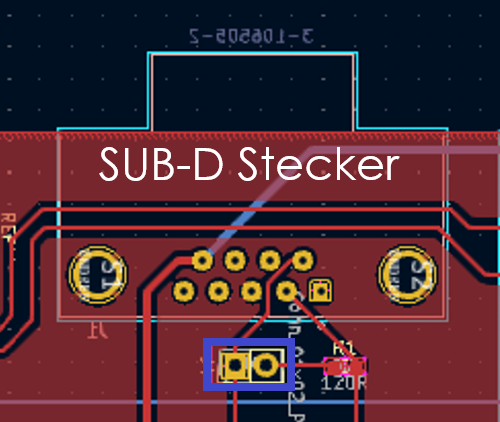
\includegraphics[width=0.5\textwidth]{img/SUB_D_zuschaltbarer_widerstand.png}
\captionof{figure}{SUB-D Stecker und Terminierungswiderstand}
\label{fig: SUB-D Stecker und Terminierungswiderstand}
\end{centering}

\section{Can Transciever}
\noindent Der MCP2562-E-P Transceiver spielt eine zentrale Rolle im Hardwareaufbau für die CAN-Kommunikation, indem er die Signale aus dem CAN-Netzwerk in digitale Signale umwandelt, die vom ESP32-Mikrocontroller verarbeitet werden können. Der Transceiver agiert als Bindeglied zwischen den differenziellen Signalen des CAN-Busses und den digitalen I/O-Pins des ESP32. Er wandelt die auf dem CAN-Bus empfangenen Hoch- und Niedrigzustände (CAN\_H und CAN\_L) in logische Pegel um, die der Mikrocontroller verstehen kann. Dies ermöglicht eine reibungslose und zuverlässige Kommunikation zwischen den CAN-Geräten und dem Mikrocontroller.\\

\noindent Zur Implementierung dieser Funktion müssen die CAN\_H und CAN\_L Leitungen des MCP2562-E-P an die entsprechenden Leitungen des CAN-Busses angeschlossen werden. Die Tx und Rx Pins des Transceivers werden dann mit den entsprechenden digitalen I/O-Pins des ESP32 verbunden, um die Kommunikation zu ermöglichen. Die genaue Pinbelegung und Konfiguration ist in dem Datenblatt des Transceivers zu finden \cite{2}.\\

\section{Status LEDS}
In unserem eingebetteten System fungieren Leuchtdioden (LEDs) als visuelle Indikatoren für verschiedene Zustände des Gerätes. Ihre Hauptfunktion besteht darin, den Benutzer über den aktuellen CAN Status zu informieren. Die LEDs sind über 270-Ohm-Widerstände an den Mikrocontroller angeschlossen, um den Strom zu begrenzen, der durch die LEDs fließt. Dies schützt die LEDs vor Überstrom, der sie beschädigen könnte, und stellt sicher, dass sie innerhalb ihrer spezifizierten Stromgrenzen betrieben werden, was zu einer längeren Lebensdauer und zuverlässigeren Leistung führt.\\

\begin{itemize}
  \item \textbf{Orange LED (D3):} Die Beleuchtung dieser LED zeigt an, dass das System mit Strom versorgt wird, und dient somit als Power-On-Statusanzeige.
  \item \textbf{Rote   LED (D4):} Diese LED beginnt zu leuchten, wenn die Nachrichten auf dem angeschlossenen CAN-Bus nicht interpretiert werden können. Dies dient als Indikator für Störungen oder Fehler im CAN-System.
  \item \textbf{Grüne  LED (D5):} Die grüne LED signalisiert, dass die Nachrichten des CAN-Bus korrekt interpretiert werden und das System ordnungsgemäß funktioniert.
  \item \textbf{Blaue  LED (D6):} Diese LED beginnt zu blinken wenn eine CAN Nachricht gesendet wird.
  \item \textbf{Blaue  LED (D7):} Diese LED beginnt zu blinken wenn eine CAN Nachricht empfangen wird.
\end{itemize}

\noindent Die Ansteuerung der LEDs erfolgt direkt durch den ESP32-Mikrocontroller, der die Fähigkeit besitzt, seine GPIO-Pins (General Purpose Input/Output) als Ausgänge zu konfigurieren. Durch Programmierung des Mikrocontrollers kann jeder dieser Pins einen High- oder Low-Zustand annehmen, wobei High bedeutet, dass der Pin eine Spannung ausgibt, die ausreicht, um die LED zum Leuchten zu bringen. Der Low-Zustand hingegen unterbricht den Stromfluss, sodass die LED erlischt.\\


\section{Buttons}
\noindent In unserem System werden Taster (Buttons) als Eingabemittel für Benutzerinteraktionen verwendet. Sie ermöglichen es dem Benutzer, Steuersignale an den Mikrocontroller zu senden, der diese dann entsprechend der programmierten Logik interpretiert. Die Taster sind einfache, aber effektive Komponenten in der Mensch-Maschine-Interaktion innerhalb eingebetteter Systeme.\\

\noindent Die drei Taster sind jeweils über einen Pull-up-Widerstand an eine Versorgungsspannung (+3V3) angeschlossen. Dies sorgt dafür, dass das Signal am entsprechenden Eingangspin des ESP32 standardmäßig auf einem hohen Logikniveau (High) liegt. Wird der Taster gedrückt, schließt sich der Stromkreis, und der Eingangspin wird auf das niedrige Logikniveau (Ground) gezogen.Die zusätzlichen Widerstände (R12, R13, R14) dienen als Strombegrenzungswiderstände und schützen den Mikrocontroller vor hohen Strömen, die beim Schließen des Tasterkreises entstehen könnten. Diese Anordnung wird als Pull-up-Konfiguration bezeichnet und ist eine gängige Methode, um den Zustand eines Eingangspins zu definieren, wenn kein Signal anliegt.\\

\noindent Im Konfigurationsmodus unseres Systems ermöglichen es die Taster dem Benutzer, die Einstellungen für die Baudrate zu navigieren und zu bestätigen. Jeder Taster hat eine spezifische Rolle:

\begin{itemize}
  \item \textbf{Taster S3:} Dieser Taster ermöglicht es dem Benutzer, auf dem Display nach oben zu navigieren.
  
  \item \textbf{Taster S4:} Der Taster S4 bietet dem Benutzer die Möglichkeit, Einstellungen zu bestätigen, wie beispielsweise die Auswahl der Baudrate.
  
  \item \textbf{Taster S5:} Sollte der Benutzer im Display nach unten navigieren müssen, wird Taster S5 verwendet.
\end{itemize}


\section{Logic Level Converter}
\noindent Im Kontext eingebetteter Systeme spielt die Signalintegrität zwischen verschiedenen elektronischen Komponenten eine entscheidende Rolle. Verschiedene Bauteile operieren oft mit unterschiedlichen Logikpegeln, was bedeutet, dass die Spannung, die ein High-Signal (logische "1") repräsentiert, zwischen diesen Komponenten variieren kann. Um eine korrekte und sichere Kommunikation zwischen solchen Bauteilen zu gewährleisten, werden Logikpegelwandler eingesetzt.\\

\noindent In unserem System haben wir den Logikpegelwandler PCA9306DCTR implementiert, um eine bidirektionale Schnittstelle zwischen dem 3,3-Volt-Logikpegel des ESP32-Mikrocontrollers und dem 5-Volt-System des Displays zu schaffen. Dieser Schritt ist notwendig, da eine direkte Verbindung ohne entsprechende Anpassung der Spannungsniveaus zu einem für das Display nicht detektierbaren Signal führen würde.\\

\noindent Der PCA9306DCTR zeichnet sich durch eine Schaltung aus, die mit Transistoren und Pull-up-Widerständen ausgestattet ist. Diese Komponenten sind präzise konfiguriert, um eine nahtlose Umwandlung von Signalen zu ermöglichen: Ein High-Signal wird von der niedrigeren Spannung des ESP32 (3,3 V) auf die höhere Spannung des Displays (5 V) angehoben und umgekehrt. Diese Funktionsweise stellt sicher, dass es zu keiner Signalverzerrung oder Beeinträchtigung der Signalintegrität kommt. Der PCA9306DCTR ermöglicht so eine reibungslose und sichere Interaktion zwischen dem ESP32 und dem Display, was für die Zuverlässigkeit und Robustheit des Gesamtsystems unerlässlich ist.\\

\section{Bypass Kondensatoren}
Die Stabilität und Zuverlässigkeit der Stromversorgung sind für die Funktionalität des Systems von entscheidender Bedeutung. Um dies zu gewährleisten, werden Bypass- oder Abblockkondensatoren an den Spannungsausgängen des ESP32 eingesetzt. Diese Kondensatoren spielen eine zentrale Rolle bei der Minimierung von Spannungsschwankungen und elektrischem Rauschen, die die Leistung und das Verhalten des Systems negativ beeinflussen können.\\

\noindent \textbf{Stabilisierung der Versorgungsspannung}\\
\noindent Bypass-Kondensatoren dienen als lokale Energiereserven, die direkt an den Spannungsausgängen des ESP32 positioniert sind. Sie bieten eine schnelle Reaktionsquelle für Energie, um die Versorgungsspannung konstant zu halten, wenn der Mikrocontroller zwischen energieintensiven Prozessen wechselt.\\

\noindent \textbf{Rauschunterdrückung}\\
\noindent Elektronische Schaltungen sind anfällig für Rauschen und transiente Störungen, die von anderen Teilen der Schaltung oder externen Quellen stammen können. Die Bypass-Kondensatoren filtern effektiv das hochfrequente Rauschen heraus, indem sie es zur Masse ableiten, und verhindern so, dass es die Leistung des Mikrocontrollers beeinträchtigt.\\

\noindent \textbf{Reaktion auf Lastwechsel}\\
\noindent Der ESP32 kann plötzliche Lastwechsel erfahren, beispielsweise beim Übergang von einem niedrigen Stromverbrauchszustand zu einer hohen Rechenleistung. Bypass-Kondensatoren helfen, solche Lastwechsel zu bewältigen, indem sie sofort Energie liefern oder aufnehmen, um die Versorgungsspannung zu stabilisieren.\\

\noindent \textbf{Dimensionierung der Bypass-Kondensatoren}\\
\noindent Zwei Arten von Bypass-Kondensatoren werden typischerweise verwendet:
\begin{itemize}
  \item \textbf{Kondensatoren mit 100nF:} Diese sind für die Filterung hochfrequenter Störungen ausgelegt und sind ein Standard in vielen Schaltkreisen, die integrierte Schaltungen enthalten.
  \item \textbf{Kondensatoren mit 4,7µF:} Sie bieten eine größere Kapazität für die Energieaufnahme und sind besonders effektiv, um die Spannung bei größeren Lastwechseln zu stabilisieren.
\end{itemize}

\noindent Diese Kondensatoren ergänzen sich gegenseitig, wobei der 100nF-Kondensator schnelle, kurzzeitige Schwankungen abfängt, während der 4,7µF-Kondensator für länger anhaltende Stabilität sorgt. Die Kombination beider Typen stellt sicher, dass der ESP32 unter allen Betriebsbedingungen effizient und fehlerfrei arbeiten kann.



\section{Stückliste}

\begin{table}[htbp]
  \begin{center} % Zentriert die Tabelle
      \begin{tabular}{cccc} % Definiert die Anzahl und Ausrichtung der Spalten (hier: zwei zentrierte Spalten)
          \hline % Horizontale Linie oberhalb der Tabelle
          Name & Bauteilbezeichnung & Spezifikationen & Menge \\ % Inhalt der Tabelle, & trennt die Spalten
          \hline % Horizontale Linie oberhalb der Tabelle
          ESP32 & ESP-32 Dev Kit C V4 &  & 1\\
          Widerstand  &  & 270 Ohm & 5 \\
          Widerstand &  & 120 Ohm & 1 \\
          Widerstand &  & 1k Ohm & 3 \\
          Widerstand &  & 10k Ohm & 7\\
          Widerstand &  & 200k Ohm & 1\\
          Kondensator &  & 4.7 µF & 2\\
          Kondensator &  & 100nF & 2\\
          LED &  & & 5\\
          SUB-D Stecker & 3-106505-2 & & 1\\
          Button & B3FS-1010P & & 3\\
          CAN Transceiver & MCP2562-E-P & & 1\\
          Logic Level Converter & PCA9306DCTR & & 1\\
          Display & WayinTop 20x4 2004 LCD & & 1\\
          Display Anschluss & TWI IIC I2C LCD & & 1\\
          Leiterplatte &  & & 1\\
          \hline % Horizontale Linie unterhalb der letzten Zeile
      \end{tabular}
  \caption{Stückliste der verwendeten Bauteile}
  \label{tab:Stückliste}
  \end{center}
  \end{table}
\chapter{Software}

Die Software des Systems setzt sich aus zwei Hauptkomponenten zusammen. Zur Verarbeitung der eingehenden CAN-Nachrichten wird eine ESP32 verwendet, der auf dem espidf-Framework basiert. Dieser Microcontroller übernimmt nicht nur das Empfangen der Nachrichten, sondern zeigt diese auch auf einem LCD-Display an und stellt sie über eine REST-API zur Verfügung. Um eine benutzerfreundlichere Oberfläche zu bieten, wurde zusätzlich eine GUI entwickelt. Diese basiert auf dem von Google entwickelten Framework Flutter. Dank dieser GUI können die CAN-Nachrichten komfortabel über eine Windows-Anwendung, einen Browser oder einer App ausgelesen werden. Das Architekturbild \ref{fig:architekturbild} stellt die grundsätzliche Architektur des Systems dar. Auf die einzelnen Komponenten wird im folgendem genauer eingegangen.
\begin{figure}[h]
  \centering
  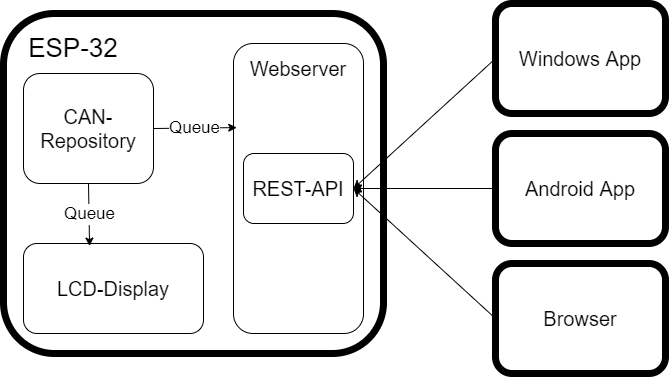
\includegraphics[width=0.8\textwidth]{img/architekturbild.drawio.png}
  \caption{Architekturbild}
  \label{fig:architekturbild}
\end{figure}


\section{ESP32}
\subsection{Architektur}
\subsubsection{Projektstruktur}
Bei der Projektstruktur \ref{fig:projektstruktur_esp} wurde sich an der Clean Architecture von Robert C. Martin orientiert \cite{martin_clean_2018}. Da diese für Objekt Orientierte Programmiersprachen ausgelegt ist, wurde die Struktur an unsere Bedürfnisse angepasst. Der Benefit der Projektstruktur ist, dass die Business Logiken, welche in den Controllern implementiert sind, von der Verarbeitung der Daten gekapselt werden. Jeder Controller ist ein FreeRTOS Task, welche die gleiche Grundstruktur, eine FSM, besitzt. Auf die FSM wird in \ref{chap:fsm} genauer eingegangen.
\begin{lstlisting}
    while (1)
    {
        switch (fsm_controller_current_state)
        {
        case STARTING:
            break;
        case CONFIGURATION:
            break;
        case OPERATION:
            break;
        }
        vTaskDelay(10);
    }
\end{lstlisting}
Der Bereich \textit{data} ist für die Verarbeitung der Daten zuständig. Hier werden die Rohdaten in geeignete Strukturen transformiert, die für die Controller leicht zu verarbeiten sind. Die Strukturen sind in \textit{models} definiert.
\begin{figure}[h]
  \centering
  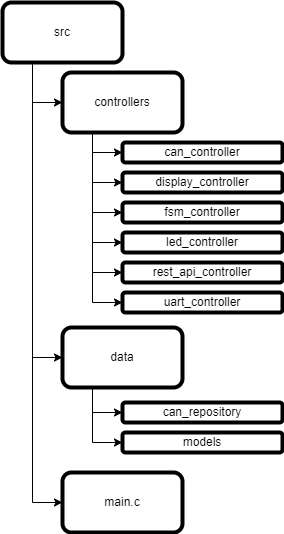
\includegraphics[height=0.7\textwidth]{img/projektstruktur.png}
  \caption{Projektstruktur ESP}
  \label{fig:projektstruktur_esp}
\end{figure}

\subsubsection{Finite State Machine}
\label{chap:fsm}
Um das Verhalten des Systems klar und strukturiert zu unterteilen, wurde eine Final State Machine (FSM) eingesetzt. Diese besteht aus den drei States \textit{STARTING}, \textit{CONFIGURATION} und \textit{OPERATION} \ref{fig:fsm}.
\begin{figure}
  \centering
  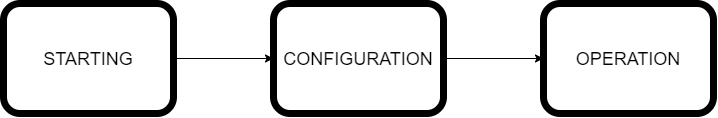
\includegraphics[width=0.8\textwidth]{img/fsm.drawio.png}
  \caption{FSM}
  \label{fig:fsm}
\end{figure}
Der State \textit{STARTING} \ref{fig:state_starting} ist für den Systemstart verantwortlich. Hierbei werden die einzelnen Controller als FreeRTOS Tasks gestartet.
\begin{figure}
  \centering
  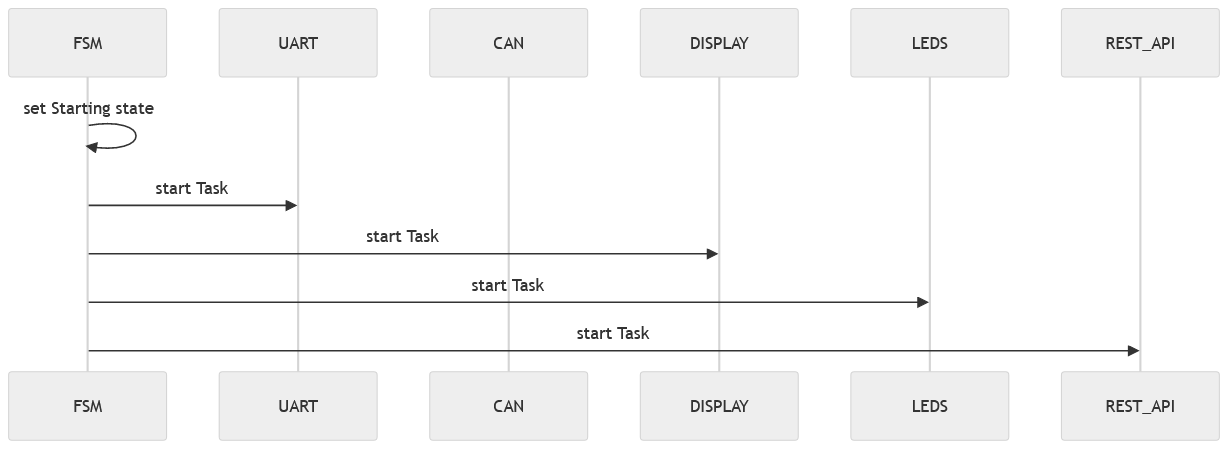
\includegraphics[width=0.8\textwidth]{img/state_starting.PNG}
  \caption{State STARTING}
  \label{fig:state_starting}
\end{figure}
Daraufhin wird in den \textit{CONFIGURATION} \ref{fig:state_configuration} State übergegangen. Hier wird das System mit den nötigen Einstellungen konfiguriert. So wird unter anderem die Baudrate des CAN Netzwerks vom User gesetzt und an den CAN Controller übertragen.
\begin{figure}
  \centering
  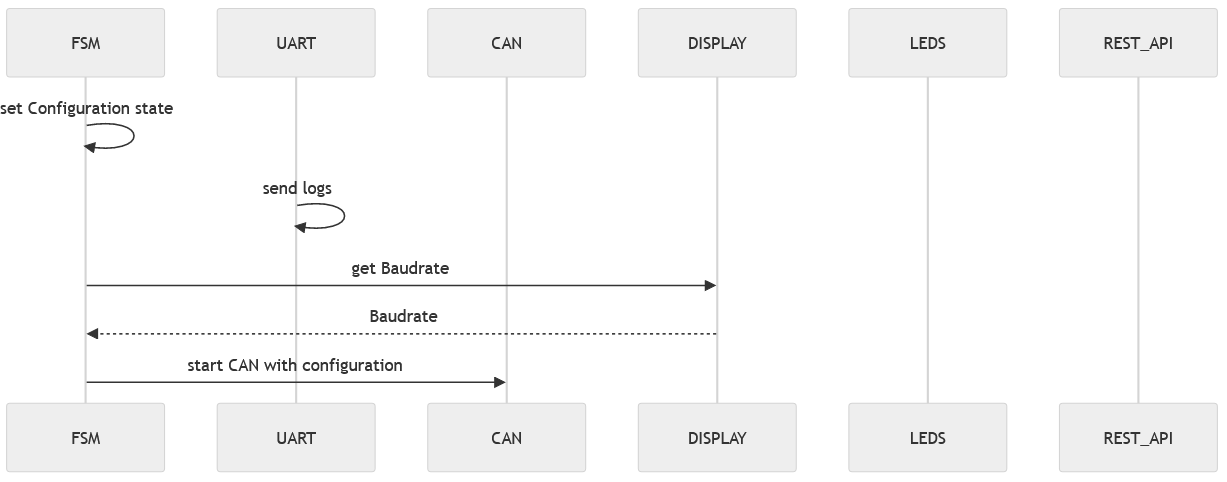
\includegraphics[width=0.8\textwidth]{img/state_configuration.PNG}
  \caption{State CONFIGURATION}
  \label{fig:state_configuration}
\end{figure}
Wenn alle Konfigurationen abgeschlossen sind, kann in den \textit{OPERATION} \ref{fig:state_operation} State gewechselt werden. In diesem Zustand wird das CAN Netzwerk laufend auf Funktionalität geprüft. Außerdem wird auf ankommende CAN Nachrichten gelauscht. Das Resultat der Funktionalitätsprüfung wird anschließend dem LED Controller mitgeteilt, sodass dieser die richtigen LEDs schalten kann. Wenn eine CAN Nachricht angekommen ist, wird diese vom CAN Repository verarbeitet und auf die jeweiligen Queues aufgeteilt. Anschließend steht die Nachricht dem LED Controller, dem Display Controller und dem REST API Controller zur Verfügung. Jetzt können von den Controllern die richtigen LEDs geschalten, sowie das Display und die REST API mit der neuen Nachricht aktualisiert werden.
\begin{figure}
  \centering
  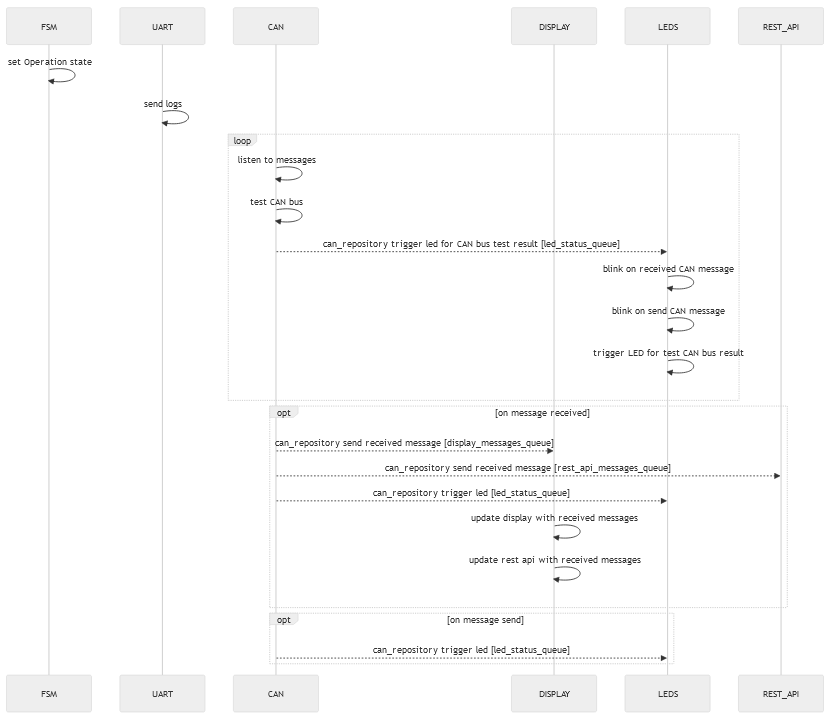
\includegraphics[width=0.8\textwidth]{img/state_operation.PNG}
  \caption{State OPERATION}
  \label{fig:state_operation}
\end{figure}

\subsection{Wichtige Komponenten}
\subsubsection{CAN Repository}
Ein zentraler Baustein der Software ist das CAN Repository mit den definierten Datenmodellen. Laut Robert C. Martins Clean Architecture \cite{martin_robert_c_clean_2012} sollten für eine saubere Software Architektur Interface Adapter implementiert werden. Die Interface Adapter sind für die Konvertierung der Daten zwischen Data Source, in unserem Fall dem CAN Controller, und den UseCases, bei uns LEDs, Display und REST API, zuständig. Durch die vorhergehende Datenkonvertierung können sich die UseCases ihrer einzigen Aufgabe, nämlich die Anzeige der Daten widmen. Mit dieser Implementierung ist auch das Single Responsibility Principle der SOLID Prinzipien erfüllt \cite{martin_robert_c_solid_2020}. Dementsprechend wurde für jeden Controller (LED, DISPLAY und REST\_API) ein entsprechendes Datenmodell definiert. Diese Datenmodelle enthalten außschließlich Informationen, die für die Anzeige der Daten mit dem jeweiligen Controller nötig sind.
\begin{lstlisting}
    #LED
    struct Led
    {
        enum Leds gpio;
        enum LedValue value;
    };
    
    #DISPLAY
    struct MessageItem
    {
        int id;
        char text[21];
    };
    
    #REST_API
    struct CanMessage
    {
        int64_t micros;
        twai_message_t message;
    };
\end{lstlisting}
Für die Konvertierung der Rohdaten des CAN Controllers, in die jeweiligen Datenmodelle wurde im CAN Repository, je eine Funktion implementiert. Danach wird das konvertierte Datenmodell in die jeweilige Queue geschrieben.
\begin{lstlisting}
static struct MessageItem twai_message_to_display_message_item(twai_message_t twai_message)
{
    struct MessageItem message_item;

    message_item.id = twai_message.identifier;

    const int index_data_start = 9;
    sprintf(message_item.text, "0x%lX", twai_message.identifier);
    const int needed_whitespaces = index_data_start - strlen(message_item.text);

    for (int i = 0; i < needed_whitespaces; i++)
    {
        strcat(message_item.text, " ");
    }

    int arrayLength = sizeof(twai_message.data) / sizeof(twai_message.data[0]);

    for (int i = 0; i < arrayLength; i++)
    {
        char item[10];
        snprintf(item, sizeof(item), "%d", twai_message.data[i]);
        strcat(message_item.text, item);
    }

    return message_item;
}

static struct CanMessage twai_message_to_can_message(twai_message_t twai_message)
{
    struct CanMessage can_message;

    int64_t uptime_micros = esp_timer_get_time();
    can_message.micros = uptime_micros;
    can_message.message = twai_message;

    return can_message;
}

extern void can_repository_distribute_received_message(twai_message_t received_twai_message)
{
    struct MessageItem received_message_item = twai_message_to_display_message_item(received_twai_message);
    xQueueSend(display_messages_queue, &received_message_item, 1);

    struct CanMessage received_can_message = twai_message_to_can_message(received_twai_message);
    xQueueSend(rest_api_messages_queue, &received_can_message, 1);

    struct Led led_blue_receive = {LED_BLUE_RECEIVE, LED_ON};
    xQueueSend(led_status_queue, &led_blue_receive, 1);
}
\end{lstlisting}
Durch diese Implementierung unter Beachtung der Clean Architecture und SOLID Prinzipien ist die Data Source von den UseCases gekapselt. Somit ist eine leichte Wartbarkeit und Erweiterbarkeit der Software gewährleistet.

\subsubsection{Display}
Das Display verfügt aktuell über zwei verschiedene Anzeigemöglichkeiten. Zum einen kann ein Menü mit beliebigen Menüeinträgen erstellt werden, zum anderen können die aktuellen CAN Messages angezeigt werden. \\
Um die Software bei Bedarf mit weiteren Menüs einfach erweitern zu können wurde das \textit{menu\_presentation} Modul so gestaltet das ein beliebiges Menü erstellt werden kann. So kann ein Array bestehend aus \textit{MenuItem} Elementen und eine Funktion \textit{void (*func\_enter)(int)} übergeben werden, welche bei betätigen des \textit{ENTER} Buttons ausgeführt wird.
\begin{lstlisting}
struct MenuItem
{
    u_int8_t id;
    u_int8_t is_selected;
    char text[50];
    void *value;
};
\end{lstlisting}
\begin{lstlisting}
extern void menu_presentation_show(i2c_lcd1602_info_t *lcd_info, struct MenuItem menu[], int menu_size, void (*func_enter)(int), enum Button button_pressed, int initial_show)
{
    char selected_string[52] = "> ";

    if (button_pressed >= 0 || initial_show)
    {
        handle_button_pressed(button_pressed, menu, menu_size, func_enter);

        i2c_lcd1602_reset(lcd_info);
        for (int i = 0; i < menu_size; i++)
        {
            i2c_lcd1602_move_cursor(lcd_info, 0, i);

            if (menu[i].is_selected)
            {
                strcat(selected_string, menu[i].text);
                i2c_lcd1602_write_string(lcd_info, selected_string);
            }
            else
            {
                i2c_lcd1602_write_string(lcd_info, menu[i].text);
            }
        }
    }
}
\end{lstlisting}
In der aktuellen Implementierung ist ein Menü zur Auswahl der Baudrate implementiert.
\begin{lstlisting}
menu_presentation_show(lcd_info, baudrate_menu, baudrate_menu_size, baudrate_menu_send_baudrate, button_pressed, false);
\end{lstlisting}
Für die Anzeige der CAN Nachrichten auf dem Display wurde ein Algorithmus entwickelt, der sicherstellt, dass sich das Display nur aktualisiert wenn nötig \ref{fig:display_controller_show_messages}. Mit dieser Implementierung wird ein Flackern des Displays vermieden. Ereignisse, die ein neuladen des Displays auslösen sind, der Empfang einer neuen CAN ID oder eine Änderung des Data Segments einer bereits enthaltenen CAN ID. Außerdem ist es möglich mit den Buttons nach oben und unten zu scrollen, um mehr als vier CAN IDs auf dem vier zeiligen Display anzeigen zu können. Auch hier wird das Display aktualisiert.
\begin{figure}
  \centering
  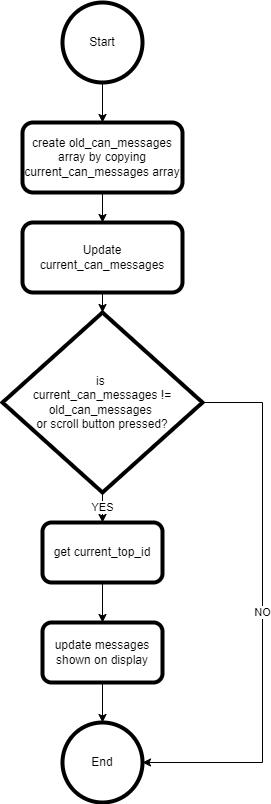
\includegraphics[height=0.8\textwidth]{img/display_controller_show_messages.png}
  \caption{Algorithmus um CAN Messages anzuzeigen}
  \label{fig:display_controller_show_messages}
\end{figure}
\subsubsection{REST API}
Um die aktuellen Nachrichten von extern leicht abfragen zu können wurde eine REST API zur Verfügung gestellt. Um auf die REST API zuzugreifen, öffnet der ESP32 den WLAN Access Point \textit{CAN-TO-GO}. Außerdem wird ein Webserver gestartet. Der Webserver stellt die Uri \textit{/can} zur Verfügung, auf welche über \textit{http://192.168.4.1/can} zugegriffen werden kann.
\begin{lstlisting}
    static httpd_uri_t get_can = {
        .uri = "/can",
        .method = HTTP_GET,
        .handler = can_get_handler,
        .user_ctx = NULL};
\end{lstlisting}
Auf dieser Seite werden die aktuellesten 100 CAN Nachrichten im JSON Format zur Verfügung gestellt.
\begin{lstlisting}
    {"messages" : [{"micros": 223754230, "id": 291, "ext": 0, "dlc": 8, "data": [0,0,1,1,0,0,0,0]},{"micros": 223864208, "id": 2047, "ext": 0, "dlc": 8, "data": [0,0,1,1,0,0,0,0]},{"micros": 223964351, "id": 35, "ext": 0, "dlc": 8, "data": [0,0,1,1,0,0,0,0]},...]}
\end{lstlisting}

\section{User Interface}
Da das Display für den Nutzer nur eine geringe Größe und eine eingeschränkte Funktionalität bietet, wurde ein externes User Interface entwickelt. Um mit einer Code Base das User Interface auf einer Vielzahl von Geräten bereitstellen zu können wurde als Framework \textit{Flutter} gewählt. Flutter ist ein Open-Source-Framework von Google, dass es erlaubt mit nur einer Code Basis das Projekt als Windows Applikation, als Web Applikation und als App auf mobilen Endgeräten zu compilieren. Als Programmiersprache wird \textit{Dart} eingesetzt.

\subsection{Funktionalitäten}
\begin{figure}[h]
  \centering
  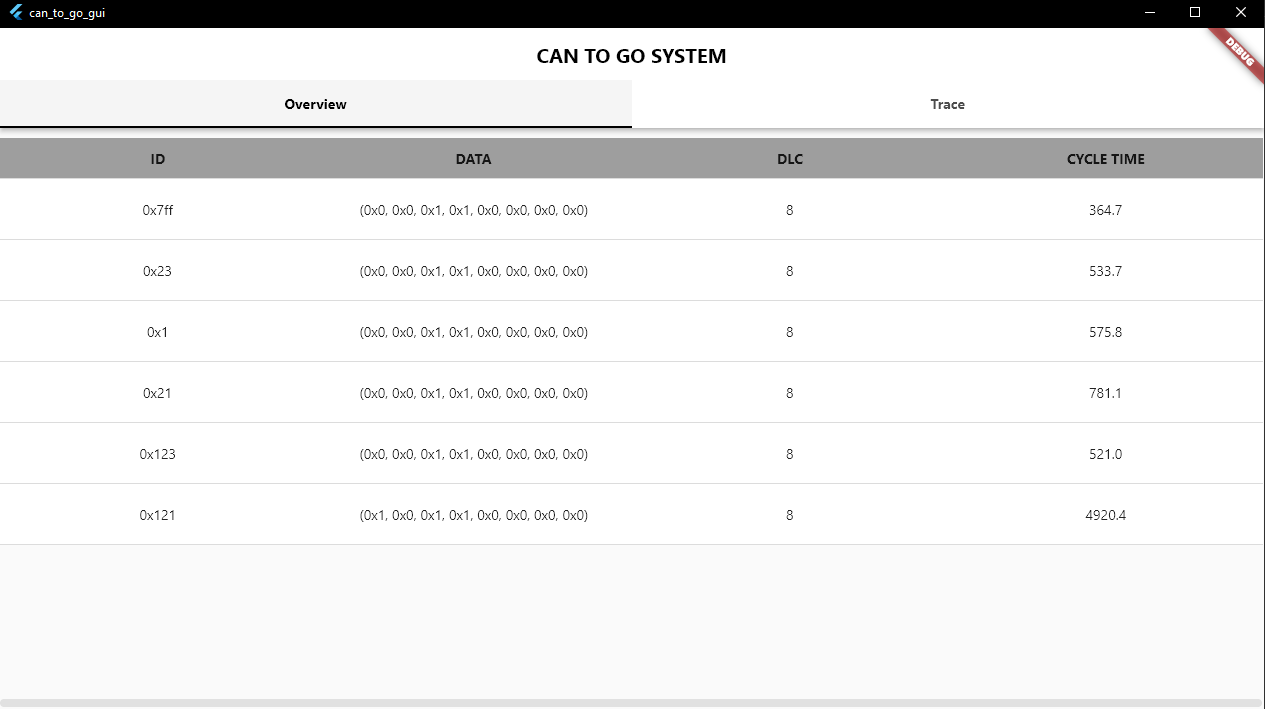
\includegraphics[width=0.9\textwidth]{img/gui_overview.PNG}
  \caption{Overview Tab}
  \label{fig:gui_overview}
\end{figure}
\begin{figure}[ht]
  \centering
  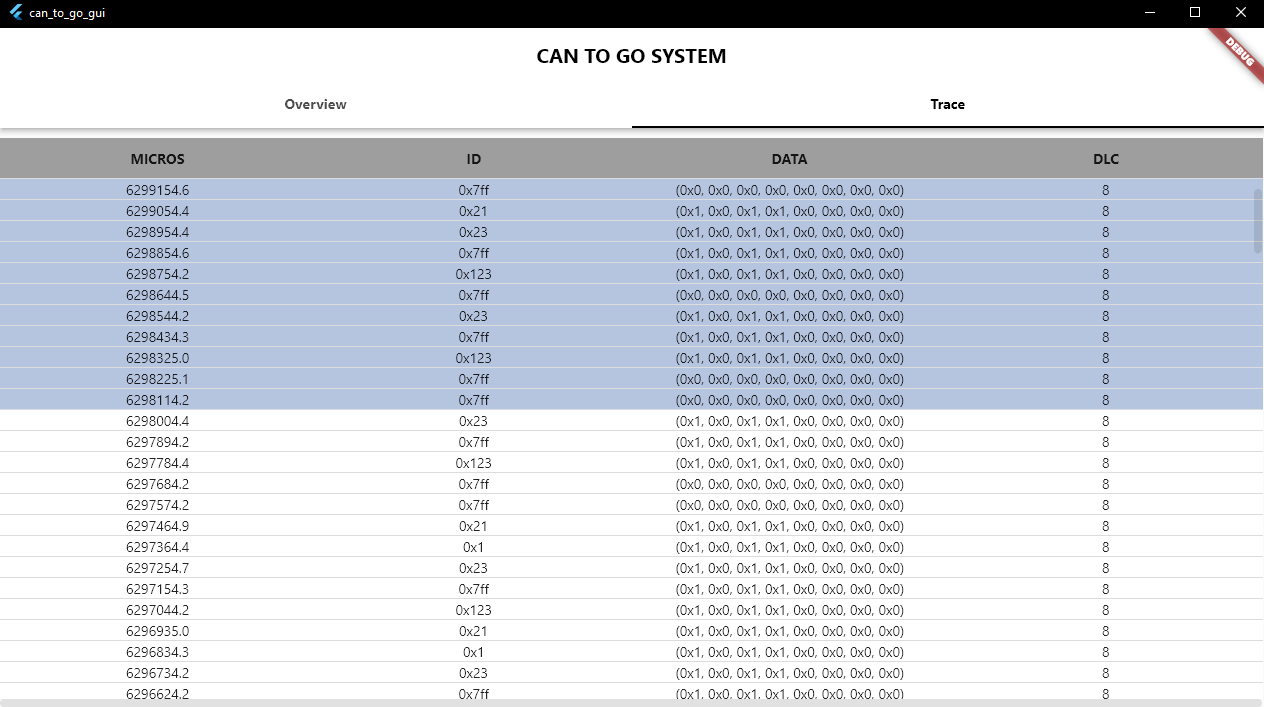
\includegraphics[width=0.9\textwidth]{img/gui_trace.PNG}
  \caption{Trace Tab}
  \label{fig:gui_trace}
\end{figure}
Das User Interface besitzt zwei verschiedene Anzeigen für den User. Zum einen gibt es ein \textit{Overview} Tab \ref{fig:gui_overview}, welches alle CAN IDs anzeigt, die empfangen wurden. Das Data Segment repräsentiert dabei immer den aktuellen Stand der jeweiligen ID. Die Cycle Time gibt darüber Auskunft, in welchem Zyklus die jeweilige CAN ID empfangen wird. \\
Außerdem gibt es die Möglichkeit über den \textit{Trace} Tab \ref{fig:gui_trace}, die letzten angekommen CAN Nachrichten zu sehen. Dabei werden die Nachrichten, die mit dem letzten Batch neu hinzugefügt wurden in einer anderen Farbe markiert, um für den User eine bessere Übersicht zu gewährleisten.

\subsection{Projektstruktur}
Bei der Projektstruktur für die GUI \ref{fig:projektstruktur_gui} wurde sich ebenfalls an der Clean Architecture von Robert C. Martin orientiert \cite{martin_clean_2018}.
Über die \textit{datasources} werden die Rohdaten von der bereitgestellten REST API gelesen und als eine Liste von \textit{CanMessageModel} zurückgegeben.
\begin{lstlisting}
    class EspRestApiRemoteDataSource {
        final String _url = "http://192.168.4.1/can";
      
        Future<List<CanMessageModel>> getCanMessages() async {
          final http.Response response = await http.get(Uri.parse(_url));
      
          List<dynamic> canMessagesJson = json.decode(response.body)["messages"];
      
          return canMessagesJson
              .map((messageJson) => CanMessageModel.fromJson(messageJson))
              .toList();
        }
      }      
\end{lstlisting}
Die Repositories sind dafür zuständig die Rohdaten in die Liste des jeweiligen Tabs zu transformieren. \\
Das \textit{CanOverviewRepository} erstellt eine Liste mit den empfangenen CAN IDs zu berechnet die Cylce Time.
\begin{lstlisting}
    Future<List<CanMessageModel>> getCanOverviewModels(bool refresh) async {
        if (refresh) {
          canMessagesCache = [];
          canMessagesUniqueIdCache = [];
        }
        final currentCanModelsBatch =
            (await espRestApiRemoteDataSource.getCanMessages()).reversed;
    
        for (CanMessageModel canMessage in currentCanModelsBatch) {
          if (!canMessagesCache.contains(canMessage)) {
            canMessagesCache.insert(0, canMessage);
          }
          if (canMessagesCache.length == 1001) {
            canMessagesCache.removeLast();
          }
        }
    
        List<CanMessageModel> currentUniqueMessages = [];
        for (CanMessageModel canMessage in canMessagesCache) {
          bool doesMessageWithIdExistInList =
              currentUniqueMessages.any((model) => model.id == canMessage.id);
          if (!doesMessageWithIdExistInList) {
            currentUniqueMessages.add(canMessage);
          }
        }
    
        for (CanMessageModel canMessage in currentUniqueMessages) {
          int index = canMessagesUniqueIdCache
              .indexWhere((item) => item.id == canMessage.id);
    
          if (canMessage.micros != 0) {
            if (index != -1) {
              canMessage.cycleTime =
                  getCycleTimeForId(canMessage.id, canMessagesCache.toList());
              canMessagesUniqueIdCache[index] = canMessage;
            } else {
              canMessagesUniqueIdCache.add(canMessage);
            }
          }
        }
    
        return canMessagesUniqueIdCache;
      }       
\end{lstlisting}
Das \textit{CanTraceRepository} erstellt eine Liste mit den letzten 200 empfangen Nachrichten und gibt zurück wie viele Nachrichten neu hinzugefügt wurden.
\begin{lstlisting}
    Future<CanTraceResult> getCanTraceModels(bool refresh) async {
        if (refresh) {
          canMessagesTrace = [];
        }
    
        final currentCanModelsBatch =
            await espRestApiRemoteDataSource.getCanMessages();
    
        int addedCount = 0;
    
        for (CanMessageModel canMessage in currentCanModelsBatch) {
          if (!canMessagesTrace.contains(canMessage)) {
            canMessagesTrace.insert(0, canMessage);
            addedCount++;
          }
          if (canMessagesTrace.length == 201) {
            canMessagesTrace.removeLast();
          }
        }
    
        return CanTraceResult(canMessagesTrace, addedCount);
      }    
\end{lstlisting}
Im \textit{presentation} Layer werden die \textit{pages} und die \textit{widgets} erstellt, die auf den jeweiligen \textit{pages} angezeigt werden. Da sowohl der \textit{Overview} Tab als auch der \textit{Trace} Tab aus einer Tabelle von CAN Nachrichten bestehen, wurde ein Widget \textit{CanTable} definiert, welches über Parameter auf das jeweilige Tab angepasst werden kann.
\begin{lstlisting}
    class CanTable extends StatelessWidget {
        final List<String> headers;
        final List<CanMessageModel> canMessages;
        final bool isOverviewTab;
        final double rowHeight;
        final int? addedCount;
    ...
    }      
\end{lstlisting}
Im \textit{Overview} Tab und im \textit{Trace} Tab wird die zuvor definierte Tabelle dann über den \textit{BuildContext} erstellt.
\begin{lstlisting}
    # Overview Tab
    Widget build(BuildContext context) {
        final List<String> headers = [
          "ID",
          "DATA",
          "DLC",
          "CYCLE TIME",
        ];
    
        return CanTable(
          headers: headers,
          rowHeight: 60.0,
          isOverviewTab: true,
          canMessages: canMessagesUniqueId,
        );
      }     
\end{lstlisting}
\begin{lstlisting}
    # Trace Tab
    Widget build(BuildContext context) {
        final List<String> headers = [
          "MICROS",
          "ID",
          "DATA",
          "DLC",
        ];
    
        return CanTable(
          headers: headers,
          rowHeight: 20.0,
          isOverviewTab: false,
          canMessages: canMessages,
          addedCount: addedCount,
        );
      }       
\end{lstlisting}

\begin{figure}
  \centering
  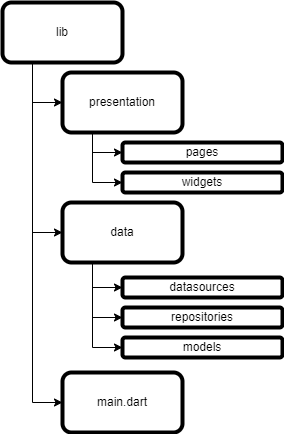
\includegraphics[height=0.7\textwidth]{img/projektstruktur_gui.png}
  \caption{Projektstruktur GUI}
  \label{fig:projektstruktur_gui}
\end{figure}

% Verzeichnis der Quellen
\printbibliography
% Verzeichnis der Bilder
\listoffigures
% Verzeichnis der Listings
%\lstlistoflistings

\end{document}